\documentclass[a4paper,12pt, english]{article}
\usepackage[top=2cm, bottom=2cm, left=2cm, right=2cm]{geometry}
\usepackage{hyperref}
%\usepackage{babel}
\usepackage{amsmath}
\usepackage{setspace}

\usepackage{subcaption}

\usepackage{listings}
\usepackage{url}
\usepackage{graphicx}


\usepackage{caption}


\usepackage{enumitem}
\setlistdepth{9}
\setlist[enumerate,1]{label=\arabic*)}
\setlist[enumerate,2]{label=\Alph*)}
\setlist[enumerate,3]{label=\Roman*)}
\setlist[enumerate,4]{label=\arabic*)}
\setlist[enumerate,5]{label=\alph*)}
\setlist[enumerate,6]{label=\roman*)}
\setlist[enumerate,7]{label=\arabic*)}
\setlist[enumerate,8]{label=\alph*)}
\setlist[enumerate,9]{label=\roman*)}

\renewlist{enumerate}{enumerate}{9}

%\usepackage{enumitem}
%\setlistdepth{9}

%\onehalfspacing

%\makeatletter
%\ifnum \@itemdepth >5\@toodeep\else
%\makeatother



\begin{document}

\title{A List of Metrics from the DMOP Ontology (94 Classes)\\ \small{\url{http://www.e-lico.org/?q=book/export/html/173}} \\ \small{\url{http://www.e-lico.org/sites/all/public/trunk/software/ontologies/dmo/DMOP/DMOP.owl}}}
\date{12 Feb 2014}
\author{By: Noureddin Sadawi}
\maketitle

\large

\begin{enumerate}

\item \textbf{AlgorithmCharacteristic}
	\begin{enumerate}
	\item \underline{BiasVarianceProfile:}
	\item \underline{ClassificationProblemType:}
	\item \underline{CoordinateSystem:}
	\item \underline{FeatureEvaluationContext:}
	\item \underline{FeatureEvaluationTarget:}
	\item \underline{HandlingOfCategoricalFeatures:}
	\item \underline{HandlingOfClassificationCosts:}
	\item \underline{HandlingOfContinuousFeatures:}
	\item \underline{HandlingOfInstanceWeights:}
	\item \underline{LearningPolicy:}
	\item \underline{RandomComponent:}
	\item \underline{RangeOfNeighborhood:}
	\item \underline{RuleInductionStrategy:}
	\item \underline{SampleHandlingForRuleInduction:}
	\item \underline{ToleranceToClassImbalance:}
	\item \underline{ToleranceToCorrelatedFeatures:}
	\item \underline{ToleranceToHighDimensionality:}
	\item \underline{ToleranceToIrrelevantFeatures:}
	\item \underline{ToleranceToMissingValues:}
	\item \underline{ToleranceToNoise:}
	\item \underline{ToleranceToWideDataSets:}
	\item \underline{TransformationFunction:}
	\item \underline{TreeBranchingFactor:}
	\item \underline{UniquenessOfSolution:}	
	\end{enumerate}
\item \textbf{DataCharacteristic}
	\begin{enumerate}
	\item \textbf{DataSetCharacteristic}
		\begin{enumerate}
		\item \underline{AverageAbsoluteFeatureCorrelation:} METAL characteristic: Average absolute correlation between continuous features.
		\item \underline{AverageCategoricalFeaturePairsMutualInformation:}  METAL characteristic: Average mutual information between pairs of categorical features. 
		\item \underline{AverageFeatureEntropy:} METAL characteristic: Average feature Entropy
		\item \underline{BetweenGroupsSumSquaresCrossProducts:} METAL characteristic: A matrix containing the difference between the matrix of total and the matrix of within-groups sums of squares and cross products.
		\item \underline{EigenValuesLinearDiscriminantFunctions:} METAL characteristic: A vector of eigen values of linear discriminant functions.
		\item \textbf{LabeledDataSetCharacteristic}
			\begin{enumerate}
			\item \underline{AverageSVMFeatureWeight:}
			\item \textbf{CategoricalLabeledDataSetCharacteristic}
				\begin{enumerate}
				\item \underline{AverageMutualInformation:} METAL characteristic: Average mutual information 
				\item \underline{AverageReliefFeatureWeight:}
				\item \underline{CanonicalCorrelationBestLinearCombination:} METAL characteristic: Canonical correlation of the best linear combination of features to distinguish between classes.
				\item \underline{ClassAbsoluteFrequencies:} METAL characteristic: Absolute class frequencies. Stored in a vector indexed by each class value.
				\item \underline{ClassCovarianceMatrices:} METAL characteristic: Class covariance matrices. Stored in a vector indexed by class and each containing a matrix of (features x features)
				\item \underline{ClassEntropy:}  METAL characteristic: Class entropy.
				\item \underline{ClassRelativeFrequencies:} METAL characteristic: Relative class frequencies. Stored in a vector indexed by each class value.
				\item \underline{ErrorRateOf1NNClassifier:}  From Mitra Basu and Tin Kam Ho. Data Complexity in Pattern Recognition. Springer, 2006.
				\item \underline{ErrorRateOfLinearClassifierLP:} From Mitra Basu and Tin Kam Ho. Data Complexity in Pattern Recognition. Springer, 2006.
				\item \underline{FeatureMutualInformationPerClass:} METAL characteristic: For each categorical feature, the mutual information between the feature and the class. It is stored in a vector indexed by each categorical feature.
				\item \underline{FeatureValueFrequenciesPerClass:} METAL characteristic: For each k value of each j categorical feature and each i class, the proportion of cases that have the k value in the j feature and belong to the i class. It is stored in a vector indexed by each categorical feature and containing a flat contingency tables that combine the values of the categorical feature with the class values. 
				\item \underline{MaximumFeatureEfficiency:} From Mitra Basu and Tin Kam Ho. Data Complexity in Pattern Recognition. Springer, 2006.
				\item \underline{MaximumFishersDiscriminantRatio:}  From Mitra Basu and Tin Kam Ho. Data Complexity in Pattern Recognition. Springer, 2006.
				\item \underline{MinimumSumOfErrorDistanceByLP:}  From Mitra Basu and Tin Kam Ho. Data Complexity in Pattern Recognition. Springer, 2006.
				\item \underline{NonLinearityOf1NNClassifier:}  From Mitra Basu and Tin Kam Ho. Data Complexity in Pattern Recognition. Springer, 2006.
				\item \underline{NonLinearityOfLinearClassifierLP:}  From Mitra Basu and Tin Kam Ho. Data Complexity in Pattern Recognition. Springer, 2006.
				\item \underline{NumberOfClasses:}
				\item \underline{ProportionOfBoundaryPoints:}  From Mitra Basu and Tin Kam Ho. Data Complexity in Pattern Recognition. Springer, 2006.
				\item \underline{ProportionPointsWithRetainedAdherence:}  From Mitra Basu and Tin Kam Ho. Data Complexity in Pattern Recognition. Springer, 2006.
				\item \underline{RatioOfAverageIntraInterDistances:}  From Mitra Basu and Tin Kam Ho. Data Complexity in Pattern Recognition. Springer, 2006.
				\item \underline{VolumeOfOverlapRegion:}  From Mitra Basu and Tin Kam Ho. Data Complexity in Pattern Recognition. Springer, 2006.
				\end{enumerate}			
			\item \underline{ContinuousLabeledDataSetCharacteristics:}
			\end{enumerate}		
		\item \underline{NoiseSignalRatio:}  METAL characteristic: Noise signal ratio
		\item \underline{NumberOfCategoricalFeatures:}
		\item \underline{NumberOfContinuousFeatures:}
		\item \underline{NumberOfFeatures:}
		\item \underline{NumberOfHOutliers:} METAL characteristic: Number of continuous features with outliers.
		\item \underline{NumberOfInstances:}
		\item \underline{NumberOfInstancesPerFeature:} From Mitra Basu and Tin Kam Ho. Data Complexity in Pattern Recognition. Springer, 2006. 
		\item \underline{ProportionOfCategoricalFeatures:}
		\item \underline{ProportionOfHOutliers:} METAL characteristic: Proportion of continuous features with outliers.
		\item \underline{TotalSumSquaresCrossProducts:} METAL characteristic: Matrix of total sums of squares and cross products of features.
		\item \underline{WithinGroupsSumSquaresCrossProducts:} METAL characteristic: matrix of within-groups sums of squares and cross products of features. 
		\end{enumerate}	 
	\item \textbf{FeatureCharacteristic}
		\begin{enumerate}
		\item \textbf{CategoricalFeatureCharacteristic}
			\begin{enumerate}
			\item \underline{FeatureClassMutualInformation:}  FeatureClassMutualInformation: For each categorical feature, the mutual information between the feature and the class. It is stored in a vector indexed by each categorical feature. [From METAL project].
			\item \underline{FeatureEntropy:} METAL characteristic: For each categorical feature, the feature entropy.
			\item \underline{FeatureFrequentValue:} A categorical value should be marked as frequent, iff it is 50\% more frequent than we would expect under a uniform distribution. (e.g. 75\% for a binary value)
			\item \underline{FeatureModalValue:}
			\item \underline{FeatureRareValue:} A categorical value should be marked as rare, iff it is 50\% less frequent than we would expect under a uniform distribution. (e.g. 25\% for a binary value)
			\item \underline{FeatureValueFrequencies:} METAL characteristic: For each k value of the feature, the value frequency. It is stored in a vector indexed by each feature value. 
			\item \underline{FeatureVeryFrequentValue:} A categorical value should be marked as very frequent, iff it is 90\% more frequent than we would expect under a uniform distribution. (e.g. 95\% for a binary value)
			\item \underline{FeatureVeryRareValue:} A categorical value should be marked as very rare, iff it is 90\% less frequent than we would expect under a uniform distribution. (e.g. 5\% for a binary value)
			\item \underline{NumberOfDistinctValues:}
			\end{enumerate}		
		\item \textbf{ContinuousFeatureCharacteristic}
			\begin{enumerate}
			\item \underline{FeatureCorrelation:} METAL characteristic: For each continuous feature, its correlation with other continuous features. Stored in a vector indexed by each continuous features.
			\item \underline{FeatureHOutlier:} METAL characteristic: For each continuous feature, the ratio between the standard deviation and the standard deviation of alpha trimmed mean. If the standard deviation is 0, then the ratio is set 1.
			\item \underline{FeatureMaximumValue:}
			\item \underline{FeatureMeanValue:}
			\item \underline{FeatureMinimumValue:}
			\item \underline{FeatureStandardDeviation:}
			\end{enumerate}		
		\item \underline{NumberOfMissingValues:}
		\item \underline{ProportionOfMissingValues:}
		\end{enumerate}
	\end{enumerate}
\item \textbf{HypothesisCharacteristic}
	\begin{enumerate}
	\item \underline{Interpretability:}
	\item \textbf{ModelCharacteristic}
		\begin{enumerate}
		\item \underline{ModelComplexity:}
		\item \underline{ModelPerformance:}
		\end{enumerate}	
	\item \underline{PatternSetCharacteristic:}
	\end{enumerate}	
\end{enumerate}
\newpage

\begin{figure}[h]   
  \centering 
  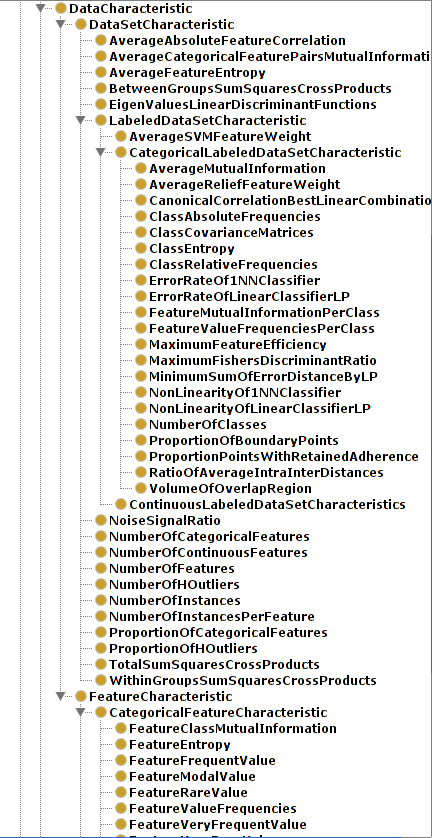
\includegraphics[width=0.75\textwidth]{../../figs/dmop1}
  \caption{}
  \label{fig:dmop1}
\end{figure}

\begin{figure}[h]   
  \centering 
  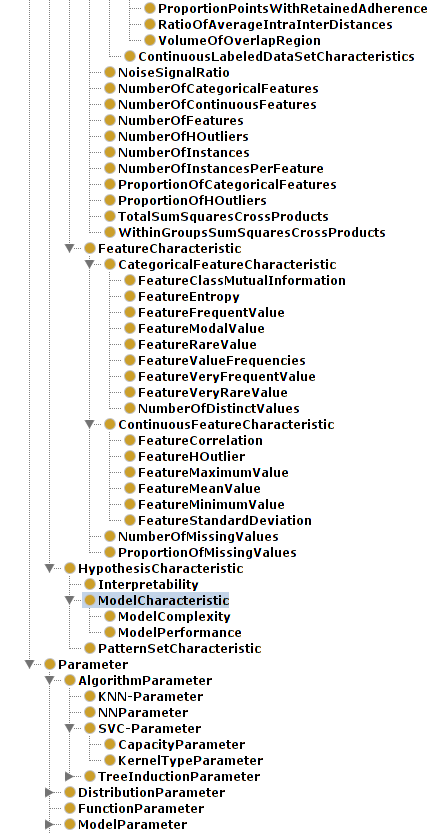
\includegraphics[width=0.75\textwidth]{../figs/dmop2}
  \caption{}
  \label{fig:dmop2}
\end{figure}

\begin{figure}[h]   
  \centering 
  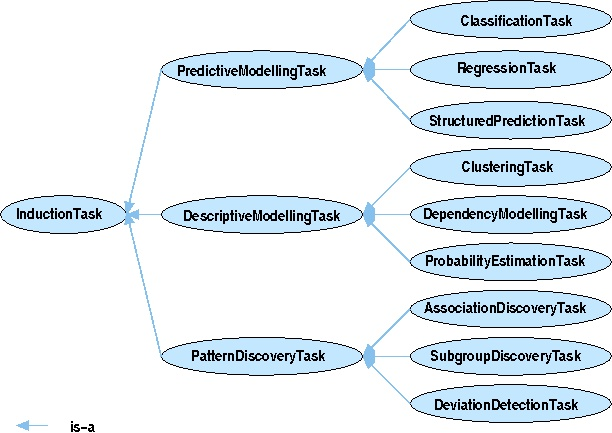
\includegraphics[width=0.75\textwidth]{../figs/dmop-task-hierarchy}
  \caption{dmop-task-hierarchy}
  \label{fig:dmop-task-hierarchy}
\end{figure}


\begin{figure}[h]   
  \centering 
  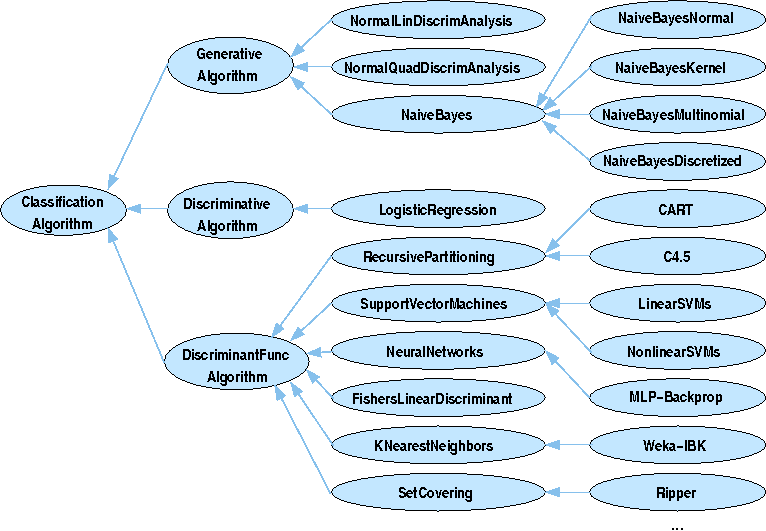
\includegraphics[width=0.95\textwidth]{../figs/dmop-classif-algo-tree}
  \caption{dmop-classif-algo-tree}
  \label{fig:dmop-classif-algo-tree}
\end{figure}

%\begin{figure}[h]   
%  \centering 
%  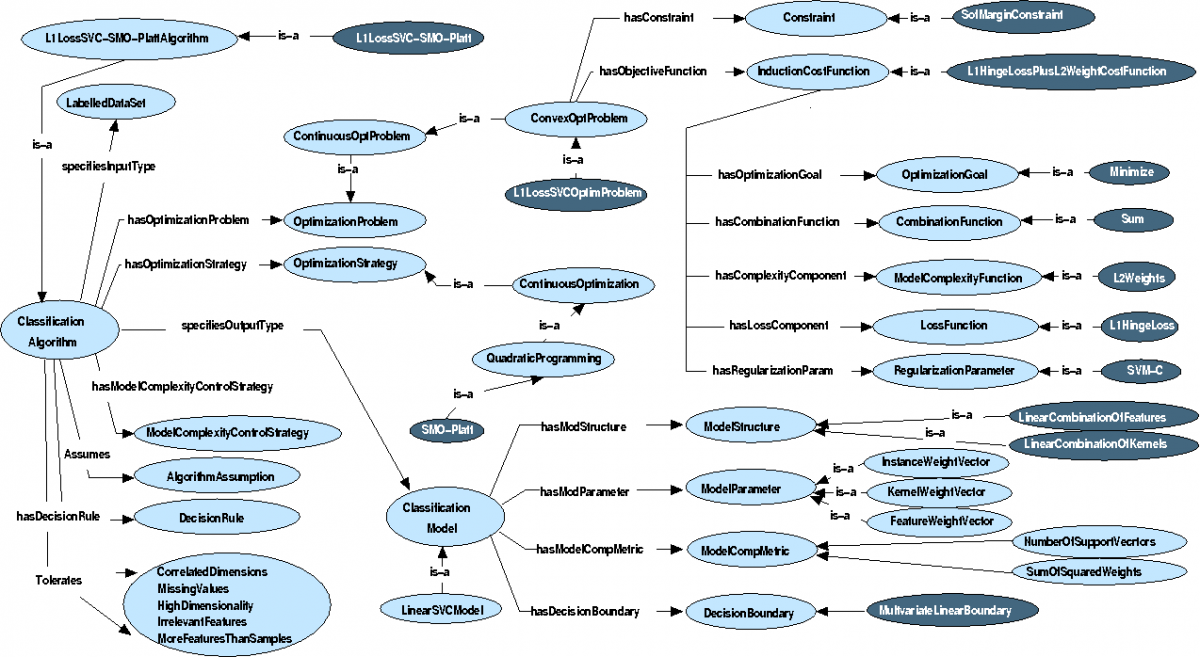
\includegraphics[width=0.95\textwidth]{../figs/dmop-SVC-algo-model-properties-all}
%  \caption{dmop-SVC-algo-model-properties-all}
%  \label{fig:dmop-classif-algo-tree}
%\end{figure}

\newpage
\begin{figure}[h]
  \centering
  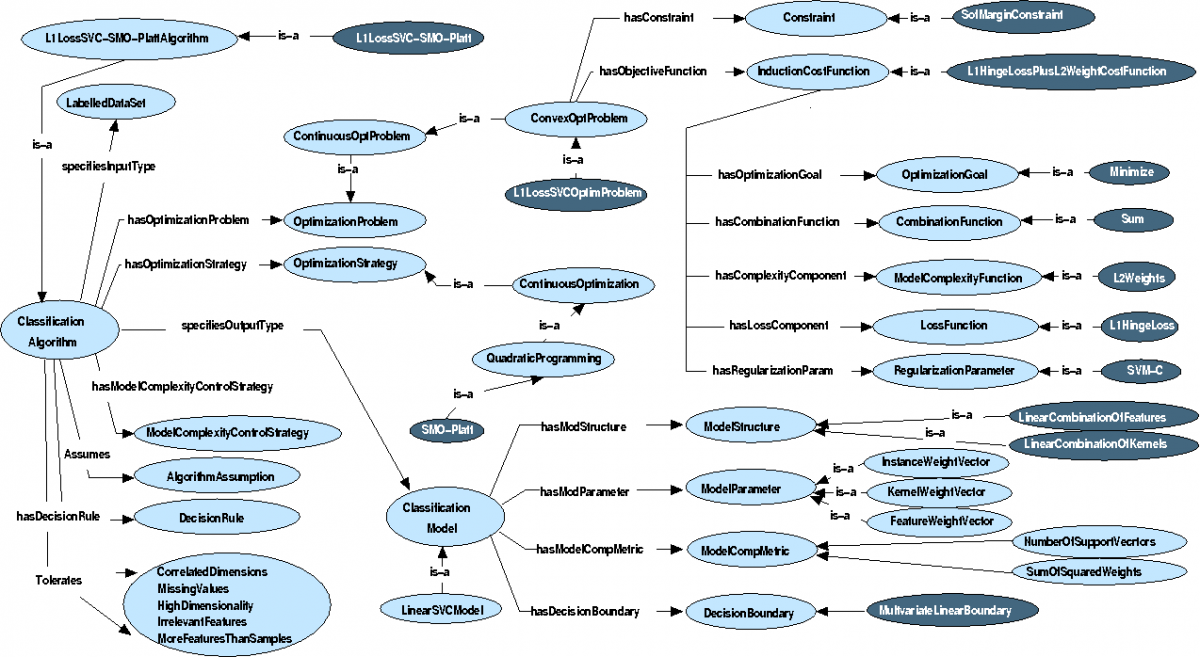
\includegraphics[height=0.45\textheight, angle=90]{../figs/dmop-SVC-algo-model-properties-all}
  \caption{dmop-SVC-algo-model-properties-all}
  \label{fig:dmop-classif-algo-tree}
\end{figure}

\end{document}
